\chapter{Solution}
\label{chapter-solution}

\section{Current publishing conventions}
\label{publishing-conventions}

Although there is no set standard on how to publish plugins, conventions have emerged over time.
Taking advantage of them is the first step towards standardizing distribution.

There are three websites where either the important ones or the majority of plugins are found:
\begin{itemize}
    \item \textbf{AlliedModders forums} -- official forums of SourceMod, usually there exists a corresponding thread, regardless where the files are hosted,
    \item \textbf{GitHub} -- preferred by some developers, either to upload binaries directly to repositories or have them posted in the \textit{Releases} section,
    \item \textbf{LimeTech} -- third-party website hosting high-traffic SourceMod extensions, owned by one of the major contributors.
\end{itemize}

\subsection{AlliedModders forums}
\label{alliedmodders-formus}

The official forums are the main source of advertising for developers, thus a sure way to find plugins.
A thread dedicated to a release of one, either hosts the files as its attachments or instructs readers where to download them from.
All addons posted on the forums must adhere to the SourceMod license, GNU General Public License, version 3.
This license applies to derivative works as well \cite{sourcemod-license}, which means that source must be provided along with distribution.

Because of this the forums have a unique feature available to developers when posting their work.
If a file is the source of a plugin (\textit{.sp} extension), it will automatically be compiled by the online compiler and displayed next to the source attachment.
While convenient, it is quite limited.
Should a plugin make use of libraries outside of the standard, the compilation will fail.
In such cases, the developer needs to compile the plugin themselves and upload it as a separate attachment.
Each are given and identified by a unique ID, which is utilized for downloading by being present in the URL\@.
Unfortunately, there is no API to parse them.

\subsection{GitHub}

GitHub is a preferable alternative to the forums as a file host by many developers.
For that, they mostly use the \textit{Releases} feature of the service but may store binary files along with everything else.
In case of the latter, there exists a URL which will always point to the latest version of any file in the repository.
A similar URL may exist pointing to a file in the \textit{Releases} section, but only for a specific release.
Therefor, if anyone wishes to programmatically fetch a file uploaded in the latest release, the GitHub API must be utilized.
It is then possible to iterate all the uploaded assets and read their names or URLs, among other properties.

\subsection{LimeTech}

LimeTech is not used by the public but rather a single developer, who also is a major contributor to both SourceMod and SourcePawn.
The website hosts files for many popular extensions, making it worthwhile to consider when finding the way to standardize distribution.

Like the forums and GitHub, it lacks a URL to download the latest publication of a project from.
And due to a lack of an API, one must resolve to scraping.
All the project releases hosted on the website are archives.
They are kept on pages of their own, in a three-column table of operating systems to specific versions.
A caveat here may be that a cell is empty, either because a certain release for a specific system is not out yet, or is simply not supported.
Thus a traversal of the table is required to find the next, latest one available.

\subsection{Other websites}

Because of the heuristic nature of the solution for standardizing distribution, support for all websites is impossible.
The top three mentioned ones are where all plugins are found, save for a few exceptions.
And all of them require a dedicated solution in order to fetch the files.

Having said that, the only information that is needed about a file is its name and download URL\@.
If both are provided as a single string of data, it can be utilized to implement a generic solution agnostic of the website.
This generic solution must not rely on any sort of API or a scraping method.
It may only download a file from a specific URL and save it under appropriate name and directory.
Limited of a solution as it is, it opens up possibility to support a whole range of websites.

A notable example here is BitBucket, an alternative to GitHub.
BitBucket has a \textit{Downloads} section, where each file is addressed by name.
Because of this, it is trivial to provide download URLs for the latest version of published files that need no specific processing.
Unlike attachments in case of the official forums, for example, which are required to be scraped.
Likewise, any website with a similar simplistic functionality is integrable with.

\section{AlliedModders' database}

When a developer creates a thread on AlliedModders to promote their plugin, they are asked to fill a short form about it.
This form contains fields such as the description, category, or applicable games.
Upon submittal, the thread is assigned a unique ID under which the plugin's metadata is saved in the forums' database.
They are then displayed along with this plugin ID in a header unique to threads in the \textit{Plugins} section of the forums.
Underneath, the author attaches applicable files, or points where to download them from.

For the vast majority of plugins, a thread is guaranteed to exist and the database is a promising source of metadata about plugins.
Unfortunately, it may not be used for four main reasons:
\begin{enumerate}
\item
No API to read from the database is available to third-parties.
Developing it would require support from the website maintainers, and although sought after, cannot be relied upon in early stages of the project.
\item
Post attachments are not tied to the plugin ID\@.
At best, they may be scraped after finding the associated thread.
Not to mention the fact, that the file download URLs need not be present in the post at all.
\item
There still is the problem of a non standardized way of installing the plugins.
By no means can the author's instructions be utilized for automating the process.
\item
Plugin ID may not exist for every installable addon for SourceMod.
Though ill-advised and rare, the author is not required to make a thread should they want to publish their work on other websites only.
Furthermore, SourceMod extensions have their own section, unrelated completely to that of plugins'.
There, no plugin ID or database entry is present.
And considering extensions have an analogous installation process and may be dependencies to other addons, they are worth supporting.
Lastly, in exceptionally rare situations, an extension may be simplified to become a plugin, and moved to the \textit{Plugins} section.
No database triggers will run, and it will be left as an atypical plugin lacking its ID.
\end{enumerate}

To combat the above issues, a custom database is set up.

\section{SourceMod Addon Manager database}
\label{smamdb-main}

As per every package manager, there exists a corresponding repository of software packages.
For a solution to SourceMod community's distribution problem, such a repository may not host files.
What it can store is the data about files which constitute a package, and where they can be downloaded from.
The crucial part is defining the format of metadata to fit plugins which are distributed across the three aforementioned websites.

Anyone should be able to describe a plugin to the system, regardless whether it is self-developed or not.
One of the most important concepts of the project is not requiring any action from other developers.
As such, the maintainer is separated from the author.
After providing the plugin specification, the rest should be taken care of automatically.
For instance, if the author releases a new version, it should not require any update from the side of the maintainer.
The plugin data is parsed by the client application, which should be able to fetch the most recent version, adapting the method to the website it detected.

To properly define a package, the following metadata must be provided, for specific reasons:
\begin{enumerate}
    \item \textbf{Name} -- Unique, case-insensitive name of the plugin; for identification, installation and searching.
    \item \textbf{Author} -- Name the original author goes by, which may differ from the maintainer; for searching.
    \item \textbf{Description} -- Short description of the idea behind the plugin; for searching.
    \item \textbf{Category} -- Category name as it appears on the AlliedModders forums; for searching.
    \item \textbf{Plugin ID} -- Plugin ID number as it appears AlliedModders forums' plugin's thread; for possible future integration.
    \item \textbf{Base URL} -- URL associated with the plugin; for installation.
    \item \textbf{Files} -- Paths and filenames defining an plugin; for installation.
    \item \textbf{Games} -- Multiple choice field defining which games the plugin works for, may be all; for searching.
    \item \textbf{Dependencies} -- Names of other plugins which this plugin is dependent upon; for installation.
\end{enumerate}

\subsection{Fields utilized for searching}

Optional but equally as important aspects of the database are its search capabilities.
Akin to AlliedModders' database, there exist fields like description, category or games.
The category is a single choice list: \textit{Admin Commands}, \textit{Fun Stuff}, \textit{Gameplay}, \textit{General Purpose}, \textit{Server Management}, \textit{Statistical}, \textit{Technical/Development}.
Similarly to author, description, or games, it is used purely for searching purposes.
The applicable games could be enforced during the installation, but often so it happens that plugin works for more games than specified by the author.

\subsection{Plugin ID}

Plugin ID is as it appears on the forums.
It serves no purpose in the early stages of the project, but might be useful should the official integration come in.
Should it, there will be no need to store the author, description or category, as all three could be fetched from the forums' database.
This way, data would not be needlessly duplicated and be required to be entered twice by the person submitting.
This feature can only be supplied for plugins, as extensions or rare cases of plugins have no ID.

\subsection{Base URL}

Base URL is the first of the two most important fields of the project.
It is by this field the website will be detected by the client-side application, after which the appropriate method of parsing will be used.
Each plugin entry must have this field carefully selected based on the website by the submitter.

\subsubsection{AlliedModders}

In case of AlliedModders, this will be the URL to the post containing the files.
From there, the client is able to scrape the attachments.
It is also possible to provide a link to the entire thread, instead of only the original post, or any webpage from which post attachments can be accessed.

\subsubsection{GitHub}

As mentioned, in GitHub it is possible to provide a URL to the latest version of the file in a repository.
This is what is used in the generic solution used for unknown websites.
However, GitHub API usage is required to parse a specific file from the latest release.
Should this functionality be needed, a URL to the repository may be entered.
After that, it is trivial for the client to find the \textit{Releases} API page and fetch the files published there.

\subsubsection{LimeTech}

LimeTech in this sense is very simple.
Every project submitted there follows a standard of being an archive in a cell of a table.
All that is needed is scraping that table to find the latest version.
The project-specific page's URL is all the information the client needs to find the files.

\subsubsection{Other websites}

Base URL field for websites besides the main three is redundant.
This is because the field is used only to detect the parsing method, but none may be supported when the URL is unknown.
In such cases, the only thing left to fill is the \textit{Files} field appropriately.

\subsection{Files}

Files is the second of the two most important fields of the project.
This is the field the client uses to link attachments parsed from the \textit{base URL} to the actual placement and names of the them on the disk.
Every file here is defined manually by the addon's maintainer in the following format: \verb|<path to file>;<file identifier>|.
The two fields must be separated by a semicolon.

\subsubsection{Path to file}

This is the property that relates directly to where the file belongs on the disk, it must be unique to server installation.
For convenience purposes, it is defined to be relative to SourceMod installation root.
From here there are the shortest paths to commonly used directories, for instance, \path{mod/addons/sourcemod/plugins}.

Relative paths are supported, such as ``\verb|..|'' to go up a directory.
This is required because, as previously mentioned, addon files may not be limited to the SourceMod directories.
A possible security flaw appears here, as the maintainer can exploit this freedom to move up as many directories as they please.
This must be accounted for and limited to the server installation, such as \path{mod/}.
An enforcement is present on the client side, making it impossible to go up more than two directories.
Furthermore, it is illegal to enter any non-directory locations, such as symlinks or mounted drives.

\subsubsection{File identifier}
\label{file-identifiers}

This property relates to the attachment names retrieved from the \textit{base URL}.
If this identifier is just a name of the file, it is cross-referenced with the attachments found.
Should it match one, the URL the attachment points to will be used to download and save the file under \path{{path/to/file}/{identifier}}.

The file identifier can also be a URL\@.
In this case the retrieved attachments are not used, since the URL is already known.
It is downloaded and saved in a similar manner, whatever legal location \textit{path to file} points to.
This is the reason the explicit semicolon separation is needed, to clearly distinguish what could be either a URL or a simple file name.

There is a third possibility, in case the name of the file is not static.
The actual name itself is not prone to change, however, the may be situations when a developer includes a version number.
This happens most often when a whole project is archived but may also come up when the plugin is a single binary file.
For this purpose, the support for regex-defined file identifiers is needed.
This will ensure the version number could be dynamic.
In such case, it is possible to match against multiple attachments.
Only one may be valid, however assuming their only difference is the version number, it is trivial to compare them to retrieve the latest one.

\subsection{Dependencies}

Dependencies on the forums are for the end user to note the prerequisites, they are listed as plugin IDs linking to appropriate threads.
The dependencies field in this project are not specifically for viewing, but are rather used in the installation.
In practise, it is quite rare for a plugin to have dependency on another.
But the less often it happens, the more surprising it may be when a plugin refuses to load.

This field is simply a string of addon names separated by comma.
Just as the names themselves, the dependencies are agnostic of whether they refer to a plugin or an extension.
For implementation-specific reasons, dependency addons must be installed prior.

\subsection{Deployment}

\subsubsection{Security}

The database is set up on a virtual private server provided by \textit{Digital Ocean}.
Interaction is achieved through an web server bound to a custom domain name -- \path{smamdb.net}.
Communication with that server is end-to-end encrypted with TLS using a certificate issued by \textit{Let's Encrypt}.
This warrants three important aspects of fetching packages:
\begin{enumerate}
\item \textbf{Authenticity} ensures that the web server the client interacts with is indeed owned by a trusted party.
\item \textbf{Integrity} takes care of fetching the data fully and correctly, without falling victim to potential tampering during transfer.
\item Despite being less important in this situation, \textbf{confidentiality} keeps the connection between the client and the web server private.
\end{enumerate}

Plugins have access to many sensitive parts of the server including database connections or the file system.
Because of this, it is important to ensure authenticity of the metadata retrieved.
This, of course, does not warrant full safety as the metadata itself could lead to vulnerable endpoints.
One reason could be that the developer who is publishing their work fancies distributing it on their own website, which happens to be unsecure.
Another reason could be that the attacker had gained access to publishing or editing plugins, rendering them compromised.

By using the OAuth2 protocol, Valve provides third-party authentication mechanism against their Steam services.
It is by these mechanisms that publishers are recognised and validated, as each of them is expected to have a Steam account.
Not everyone is allowed to publish their work on the website by default.
The user must be trusted in order to have access, and that trust is granted by the owner.
Furthermore, each submission is tied to the submitter, they may edit or delete their submissions but not others'.
To reiterate, somebody may publish the plugin for the developer instead, so they are not required to have access to make use of the service.

By the end of the day, addons and the game server itself are meant to be public entities, visible and open source.
This is why confidentiality in this case is fully optional, as SourceMod officially provides means for anyone to view the running plugins.
However, a few people might find it useful should they decide to host their own database of plugins on their own machine, as explained in later sections.

\subsubsection{Interaction API}

To interact with the database the client sends GET requests to \url{https://smamdb.net/}.
For installation purposes, only the \verb|ids| parameter must be supplied, which is a single name or multiple names of addons separated by a comma.
As a response, the server provides a list of JSON objects representing data about each addon requested, with the following fields:
\begin{itemize}
    \item \textbf{id} -- name of the addon,
    \item \textbf{author} -- to be saved locally for displaying,
    \item \textbf{description} -- to be saved locally for displaying,
    \item \textbf{url} -- \textit{base URL} which to parse,
    \item \textbf{files} -- definition of files to be searched on said URL,
    \item \textbf{deps} -- list of dependencies, omitted if there are none.
\end{itemize}

If there is more than one dependency, the server is forced to recursively retrieve all of them.
This makes it possible to return a longer list of addon objects than requested.
Furthermore, an action is taken to ensure each addon is provided only once in the list, and not processed for dependencies again.

\subsubsection{Management interface}

SourceMod Addon Manager Database is a project consisting of more than just a database and the API to call it.
This entire endeavour is largely dependent on user support and their accessibility towards it.
Under \url{https://smamdb.net/interface/} a button can be found which directs users to a Steam website in order to validate their authenticity.
After logging in through Steam, they will be forwarded to a panel showing their submitted addons, both accepted and pending, shown in Figure~\ref{fig:smamdb-panel}.

\begin{figure}[H]
  \centering
  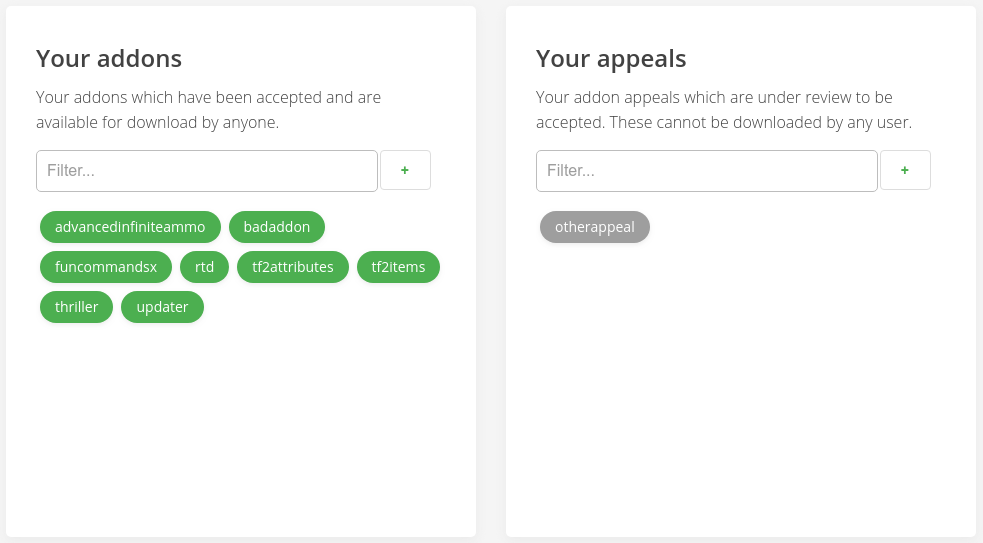
\includegraphics[scale=0.5]{smamdb-panel.png}
  \caption{SourceMod Addon Manager Database user interface panel}
  \label{fig:smamdb-panel}
\end{figure}

Pending appeals are ones awaiting a trusted user to confirm their validity.
They must be checked for correctness of the properties given but also for the trustworthiness of the submitter.
Steam API is a great help for the latter.
It can retrieve whether the user's profile is private, how long the account has existed for, or whether it had any incidents in the past, cheating or otherwise.
After this step the appeal is moved to the submission section and is available to be retrieved using the Database API\@.
At any moment the submitter is able to edit the metadata of their submissions for correction or potential upkeep requirements.

The \textit{Filter\dots} field is used to dynamically filter self submitted addons in either section by entering parts of their name.
Any of the shown ones may be clicked to open up an editing form, shown in Figure~\ref{fig:smamdb-editing}.
The plus button next to it brings up a menu to add a new submission, for untrusted users, this button is available only for the appeals section.
Submitting an addon is simply filling a form containing all the fields explained in Section~\ref{smamdb-main}.
This form looks exactly the same as the editing form, save for \textit{submit} button at the bottom, instead of \textit{delete} and \textit{update}.

\begin{figure}[H]
  \centering
  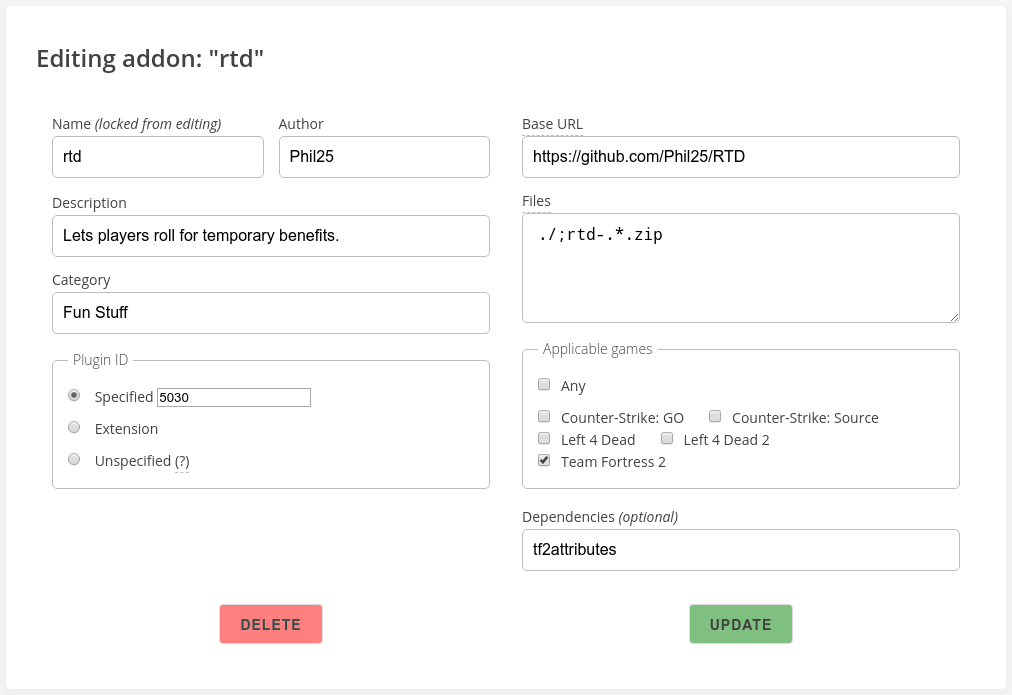
\includegraphics[scale=0.5]{smamdb-editing.png}
  \caption{SourceMod Addon Manager Database submission editing interface}
  \label{fig:smamdb-editing}
\end{figure}

\subsubsection{Self deployment}

The database website and the client application are designed to be disjoint entities.
The former exposes an API which returns data in JSON, which can be parsed by a multitude of things, due to the popularity of the format.
Likewise, calls are simple GET requests, making them trivial to be performed from many bare-bones solutions, like the \verb|curl| program.
The burden of implementation lays on the client application, it is where the complexity of the system is located.

The website is a completely different matter.
After all, the custom interface exists for human interaction and is not needed by the client.
For this reason, its only required function is the ability to parse a GET parameter and return the requested plugin metadata in a valid format.
This makes it possible to write a simple solution for a self host a web server.
As long as it is bound to a hostname, for example \verb|localhost|, the client application can interact with it just like it does with \url{https://smamdb.net/}.

A self hosted solution may be preferred by communities having their own repository of plugins and wish not to publicize them.
Another reason might be a plugin developer using it to quickly deploy their work on a testing server located on a different machine.
To achieve this, one may host the web server on their work computer and use SourceMod Addon Manager to retrieve and install the plugin remotely.
All that is needed is to point to client application to the right URL\@.
Many things are possible by having this flexibility.

\section{SourceMod Addon Manager}

The bulk of the complexity is contained within the client-side part of the project -- SourceMod Addon Manager (\textit{SMAM}).
It is a command line tool used to fetch and parse data from database websites, download addon files and keep track of them.
SMAM is distributed as a standalone binary natively compiled from modern, idiomatic C++ code, adhering to the latest standard, being C++17 at time of writing.
When the time comes, making use of many of the C++20 features is planned.

The target platforms are Linux, Windows and macOS, considering SourceMod itself is available on each.
To support this, the application is built with the help of a powerful, cross-platform build system utilizing CMake and Conan tooling.
CMake is a build system generator which creates and configures files for selected the build utility, such as UNIX Makefiles or Visual Studio.
Conan, being a praiseworthy supplement for CMake, additionally wraps the whole process in a cross-platform dependency management solution.

\subsection{Building}

The building operations are entirely abstracted by Conan and are split into a two step process:
\begin{enumerate}
\item
Firstly, \verb|conan install| command is run, specifying the root directory of the source code.
From this directory a file named \verb|conanfile.py| is parsed.
In it, the crucial parts of the build are defined, such as its type, the generator, or most notably, the project's dependencies.
Conan will ensure that they are available for the same target platform and architecture, as well as compiler and its version, as configured for the project.
The dependencies are downloaded to a remote location and built if the specific pre-compiled binaries are not found, should they even need be compiled.
The appropriate paths are then provided to the selected generator, such as CMake, to aid the compilation process in finding and linking the libraries.

\item
The execution of \verb|conan build| creates the generator configuration files in the current working directory.
When everything is in place, compilation of the project will be triggered, producing the binary in the designated location.
It is also possible to pass the \verb|-c| (configure) flag, to create CMake files only and not trigger the build afterwards.
\end{enumerate}

Additionally, Conan provides cross-building support, i.e., building for a different platform than the one the process happens on.
It does that through the help of profiles.
A profile is a file containing a pre-configured set of options defining the target and host platforms, or compiler and version, among many others.
The name of one can be provided during the setup stage and the rest will be taken care of by Conan.

\subsection{Tracking installed addons}
\label{tracking-addons}

There can be many game servers set up on a single machine, each having their own SourceMod directory, which in turn have their own set of installed addons.
Files of such addons can be split up across different directories over the server repository, which makes them non-trivial to be detected.
Because of this, SMAM keeps track of addons it has installed itself, as only then it may know all the relevant files.
It does that by storing their metadata in a local file named \verb|.smamdata.json|, in the aforementioned SourceMod's root directory.
Locally stored data is not a perfect one-to-one representation of the one stored remotely in the public database (as described in Section~\ref{smamdb-main}).
It is, however, very similar.
This allows the local and remote storage to be parsed using the same mechanism with minor adjustments, saving a lot of logic complexity.
Namely, the shared fields are \textit{id}, \textit{author}, \textit{description}, \textit{files} and \textit{deps}.

However, one more field is present only locally -- \textit{explicit}.
It is a boolean property which specifies whether the user requested that addon themselves or it was installed as a dependency outside user's instructions.
This ensures that during the removal process, all implicitly installed addons which are no longer dependent on are cleaned accordingly.

Storing a file on the disk comes with a few caveats.
It must be read and updated every time an operation is executed, which makes it vulnerable to random IO errors.
It may also fall victim to user tampering, which could easily invalidate the format.
These issues are addressed in the following ways:
\begin{enumerate}
\item
Placing a period at the beginning of the file in UNIX-based filesystems effectively hides it.
Making \verb|.smamdata.json| visible only during explicit searches.
\item
The storage file is saved in conjunction with \verb|.smamdata.json.bak|, which is its twin copy.
\item
In the root of \verb|.smamdata.json| two fields are present -- \textit{data} and \textit{hash}.
While \textit{data} is the main field from which metadata for installed addons is retrieved, the latter is its hash value.
After every saving and loading operation this value is verified.
In case a mismatch is found, a recovery using \verb|.smamdata.json.bak| is attempted.
\end{enumerate}

\subsection{Networking implementation}

Any network interaction is achieved with the help of cURL, a versatile, cross-platform C library supporting a wide range of protocols.
Each network request is accompanied by a specific user agent, generated each build using the following formula:

\begin{figure}[htp]
\centering
\verb|SourceMod Addon Manager/{major}.{minor}.{patch}-{revision}|
\end{figure}
Where \verb|{major}|, \verb|{minor}| and \verb|{patch}| are consecutive fields adhering to the semantic versioning formatting standard.
Additionally, \verb|{revision}| is provided to indicate the commit number.
For convenience purposes, this further aids the receiver in being able to pin point down the exact calling code.

Currently, the only networking functionality is downloading JSON data from a database, HTML code from websites needing scraping and files from various sources.
For these purposes, the only protocols used are HTTP or HTTPS, as only interaction from publicly available sources is needed.
The cURL library opens up possibilities for future implementations of interacting with more private sources, over protocols such as FTP or SSH.

\subsection{Fetching addon files}
\label{fetching-files}

Due to vast differences in websites needing to be searched for files, the fetching method must be adjusted accordingly.
Additionally, it must conform to a standardized output which the rest of the program can interpret in a similar manner.
Its definition is simple:
\begin{itemize}
\item \textbf{input} -- the \textit{base URL} and file identifiers (explained in Section~\ref{file-identifiers}),
\item \textbf{output} -- a map of file names to their respective downloadable URIs.
\end{itemize}

File identifiers are used for the scraping mechanism exclusively and do not necessarily represent the final names of actual files.
And because they need to be known, the file discovery process is composed of two main steps:
\begin{enumerate}
\item retrieve every relevant file from the website, then
\item evaluate the identifiers to actual file names.
\end{enumerate}

In the first step, the chosen scraper finds files on the website, these can be attachments to a forum post or a list of assets from the latest GitHub release.
It retrieves both the actual file names and where to download them from.
However, a plugin is defined by the file identifiers as specified by users in the database, not what can be found on a website by a scraper.
As such, step two is cross-referencing those identifiers with the retrieved files, effectively filtering what is unneeded.
The identifiers are evaluated to actual file names and the corresponding download URI is assigned to them.
This process follows the given formula:
\begin{enumerate}
\item
Using the exact file identifier, find the file name.
If a match of the same name is found, retrieve the URI pointed to by it and finish.

\item
Check whether the file identifier is a valid URL by itself.
If so, disregard the data scraped from the \textit{base URL} and extract the file name from the back of the identifier then finish.

\item
Treat the file identifier as a regex pattern and use it against all files retrieved from the \textit{base URL}.
If matches are found, assume they contain a version number as part of their name, then get the most up-to-date one along with its URI and finish.
Otherwise, if the regex search returned zero hits, continue to the last step.

\item
At this point around 95\% of cases have been covered.
A few more might be still accounted for after introducing a simple solution to complete the process.
Simply treat the file identifier as a valid file name and append it to the \textit{base URL} to find the download link.

\end{enumerate}

To reference the overview of publishing conventions from Section~\ref{publishing-conventions}, three of the major websites are accounted for individually.
GitHub is taken care of because of its versatile JSON-based API, which is trivial to parse.
As for AlliedModders or LimeTech, scraping of individual pages is needed.
Luckily, HTML is syntactically very close to the XML format, making it easily traversable with XPath.
Much like regex is used for finding substrings in a short and convenient syntax, XPath is a parsing solution used for finding data in XML documents.
For instance, retrieving a list of values from the second column in a table (used for LimeTech) is simplified to a single query: \verb|//td[position()=2]|.
AlliedModders is much more tricky in this regard, and many problems must be taken under consideration, outlined under Section~\ref{alliedmodders-formus}.

It might happen that the website is not recognized and no scraper can be utilized.
In such instance nothing more can be done than jumping straight to step four of the evaluation process.
That is appending the file identifier to \textit{base URL} and hoping for the best.
This is not an ideal solution yet adds support for plethora of other websites, most notably BitBucket.
The worst that could happen is an error during installation, designed to be trivially reversible as outlined in the upcoming Section~\ref{install-command}.

\subsection{Usage}

There are four modes of operations (commands) available:
\begin{enumerate}
    \item \verb|install| -- install specified addons, i.e., fetch their metadata and download files into appropriate directories, as well as dependencies,
    \item \verb|remove| -- remove downloaded files and clean up implicit dependencies,
    \item \verb|info| -- show information about currently installed addons,
    \item \verb|search| -- query the database for specified addons.
\end{enumerate}

Choosing a mode is simply typing its name after the command, followed by a potential list of addons passed as space-separated arguments: \verb|smam install rtd|.
Only one mode is performed at a time.

\subsection{Install command}
\label{install-command}

Typing \verb|smam install| will trigger the functionality responsible for collecting addon metadata and downloading files.
After the \verb|install| keyword addon IDs should be provided as space-separated arguments.
This is understandably the most complex of all the commands as it is the crux functionality of the project.

Given that administrators are free to set up as many game servers on a machine as they please, SMAM must know the location of targeted one's SourceMod directory.
Luckily, the game server has a specified, easily detectable structure, which allows for simple but efficient heuristics to be implemented.
SourceMod will be found provided the application is executed anywhere within the \textit{mod} directory, the root of server files.
Users are also able to specify the path themselves using the \verb|-d [--destination]| flag, with which the same method will be used to find the correct folder.
All the operations henceforth will be performed relative to SourceMod's root directory.

The installation process consists of five steps:
\begin{enumerate}
\item
A GET request is performed to the website pointed to by the \verb|--db-url| flag, defaulting to \url{https://smamdb.net/} if left unspecified.
This request is supplied with a variable named \verb|ids|, consisting of comma separated list of addon IDs provided by the user.
In accordance with Section~\ref{smamdb-main}, requested addon metadata is returned in the JSON format.
The data is stored by the application to be used later during the installation process.

\item
The \verb|.smamdata.json| file is read, providing information on currently installed addons.
With it, SMAM is able to recognize whether a requested addon or addons need to undergo the installation process.
If they are found already installed, each is marked as \textit{explicit} (explained in Section~\ref{tracking-addons}) and are no longer acted upon.

\item
If an addon can be installed, a directory is created in the temporary location defined by the operating system.
This step acts as initialization of a transaction, as the process is quite error-prone and meant to be easily revertible should anything go wrong.

\item
Using the parsed addon's metadata, dependencies are iterated through, downloaded and installed; then the requested addon follows suit.
Files are fetched with the method explained in Section~\ref{fetching-files}, then placed in the temporary location.
An appropriate directory structure is created along with each file, constructing a replica of the actual server structure.
Should installation of any dependency or the addon itself encounter an error, the process ends.

\item
Transaction is committed by overlaying the temporary folder with the actual one, overwriting any files.
This step's logic is largely provided by the operating system, through the standard library.
The installation process moves on to the next addon ID specified by the user, ends if there is none.
\end{enumerate}

\subsection{Remove command}

Correspondingly to installation, \verb|smam remove| cleans the files from the disk and the local cache.
Additionally, it takes care of removing every dependency which has been installed alongside the specified plugin.
To remove a dependency plugin, the following three conditions must be satisfied:
\begin{enumerate}
\item
The plugin must have been installed automatically without user's explicit command.
Supposing \verb|A| is dependent on \verb|B|, executing

\begin{figure}[htp]
\centering
\verb|smam install A && smam remove A|
\end{figure}

will install then remove \verb|B| as well.
However, if \verb|B| has been specified during installation alongside \verb|A| or installed separately, it will not be removed.

\item
The plugin must not be required by any other one, i.e., the number of plugins in need of that dependency, excluding itself, must be qual to one.
Appropriate checks are in place to take care of various edge cases.
For instance, a situation in which plugin \verb|A| depends on \verb|B| and \verb|B| depends on \verb|A|, removing \verb|A| is not posing a difficulty.

\item
The user has not passed the \verb|--no-deps| flag, which forces the application not to delete any dependnecies.

\end{enumerate}

\subsection{Info command}

When the user types \verb|smam info|, the application shows a list of installed plugin names in a compact manner.
In case the command is followed by a list of plugin names, more detailed information is displayed about each.
This command queries only the local database and is used to retrieve all kinds of information about installed plugins, including:

\begin{itemize}
    \item the name of the plugin,
    \item its author,
    \item its description,
    \item whether it has been installed explicitly or not,
    \item the list of files it manages, and
    \item the list of dependencies it requires.
\end{itemize}

\subsection{Options}

Among commands the user may pass options:
\begin{itemize}
    \item \verb|-h [--help]| -- prints help outlying all the commands and options;
    \item \verb|-v [--version]| -- prints version;
    \item \verb|-q [--quiet]| -- suppresses output;
    \item \verb|-f [--force]| -- forces command execution, different behaviour dependent on the command;
    \item \verb|--no-deps| -- disables automatic dependency installation/removal;
    \item \verb|--no-prefix| -- disables output prefixes indicating severity, such as information, warning or error;
    \item \verb|--no-color| -- disables coloring in output;
    \item \verb|--allow-running-as-root| -- enables running the command with root privileges;
    \item \verb|-d [--destination]| -- specify where to look for the server directory;
    \item \verb|-db-url| -- URL of the database to fetch metadata from, defaults to \url{https://smamdb.net/}.
\end{itemize}

%\subsection{Implementation}
%
%Package managing solutions are heavily procedural in nature.
%As such, TODO
%
%The application has four modes of operations, adhering (TODO: better word) to the aforementioned commands.
%Each of the modes uses derivatives (TODO: correct?) of the \verb|Operation| class as its building blocks.
%\verb|Operation|s define specific actions, for instance, one checks whether an addon has already been installed.
%They can only be run via the \verb|Executor|, a class which must be instantiated and method \verb|Run| must be chained to perform \verb|Operation|s in an order.

\section{Unsupported features}

Package managers are understandably very rich in features.
Modern solutions are equipped with version management, PGP package signing and trust system, installation from source or snapshots with rollbacks, among many more.
Those features help tremendously in server maintenance and security, however, many of them cannot be utilized in the current state of affairs around SourceMod.
The reasons are that those features are either impossible to implement, or the benefits are simply not worth the tradeoff for complexity and development time.

\subsection{Installing specific version}

With plethora of software out there, it often may happen that parts of the system are incompatible.
When using a modern package manager, those incompatibilities are immediately detected and the maintainer is promptly informed.
Version management gives the flexibility of installating a specific version of any package, often being the go-to solution.
Despite being used in an edge case situation, it is a very effective feature to have should such problems occur.

This requires the database to store a version controlled repository of package files.
Unfortunately, the SourceMod community does not have this convenience for majority of distributed plugins.
Each time a developer publishes a new version, the old one is usually lost from the public's perspective.

\subsection{Update command}

Updating is a core aspect of package managers.
However, similarly to previously mentioned lack of version control around plugin distribution, detecting new versions is non trivial.
This leaves re-installation of addons to be the best option should anyone want to update.

Luckily, an alternative solution for this already exists in a form of a plugin called \textit{Updater}.
Developers are required to provide support for it themselves by providing a text file accessible online which it then parses.
The plugin compares version strings specified in it and the one saved locally, and downloads the files marked as needing updating.
Additionally, it provides an option to schedule this process.
Despite explicit developer intervention not being the idea of SMAM, \textit{Updater} is fully compatible with it, provided the files do not change across versions.
